\documentclass[oneside, 11pt]{article}

\usepackage[T1]{fontenc}
\usepackage[utf8]{inputenc}
\usepackage[english]{babel}
\usepackage{enumerate}
\usepackage{isotope}


\usepackage{fouriernc}
\usepackage[detect-all, binary-units, separate-uncertainty=true,
            per-mode=symbol, retain-explicit-plus, retain-unity-mantissa=false]{siunitx}

\usepackage{setspace}
\setstretch{1.2}

\setlength{\parskip}{\smallskipamount}
\setlength{\parindent}{0pt}

\usepackage[headheight=14pt]{geometry}
\geometry{marginparwidth=0.5cm, verbose, a4paper, tmargin=3cm, bmargin=3cm,
          lmargin=2cm, rmargin=2cm}

\usepackage{float}

\usepackage[fleqn]{amsmath}
\numberwithin{equation}{section}
\numberwithin{figure}{section}

\usepackage{graphicx}
\graphicspath{{images/}{../../../images/}}

\usepackage{tikz}
\usetikzlibrary{shapes}
\usetikzlibrary{plotmarks}

\newcounter{Exercise}
\setcounter{Exercise}{1}
\usepackage{xcolor}
\definecolor{shadecolor}{gray}{0.9}
\usepackage{framed}
\usepackage{caption}

\usepackage{url}


\usepackage{fancyhdr}
\pagestyle{fancy}
\fancyhf{}
\rhead{\thepage}
\renewcommand{\footrulewidth}{0pt}
\renewcommand{\headrulewidth}{0pt}

\fancypagestyle{firststyle}
{
    \fancyhf{}
    \rhead{\thepage}
    \cfoot{\includegraphics[height=30pt]{HiSPARClogo}}
    \rfoot{\includegraphics[height=25pt]{CCbysa}}
    \lfoot{
\includegraphics[height=30pt]{NIKHEFlogo}}
    \renewcommand{\footskip}{50pt}
    \renewcommand{\footrulewidth}{0.1pt}
    \renewcommand{\headrulewidth}{0pt}
}

\newcommand{\figref}[1]{Figuur~\ref{#1}}

\newcommand{\hisparc}{\textsmaller{HiSPARC}\xspace}
\newcommand{\kascade}{\textsmaller{KASCADE}\xspace}
\newcommand{\sapphire}{\textsmaller{SAPPHiRE}\xspace}
\newcommand{\jsparc}{\textsmaller{jSparc}\xspace}
\newcommand{\hdf}{\textsmaller{HDF5}\xspace}
\newcommand{\aires}{\textsmaller{AIRES}\xspace}
\newcommand{\csv}{\textsmaller{CSV}\xspace}
\newcommand{\python}{\textsmaller{PYTHON}\xspace}
\newcommand{\corsika}{\textsmaller{CORSIKA}\xspace}
\newcommand{\labview}{\textsmaller{LabVIEW}\xspace}
\newcommand{\daq}{\textsmaller{DAQ}\xspace}
\newcommand{\adc}{\textsmaller{ADC}\xspace}
\newcommand{\hi}{\textsc{h i}\xspace}
\newcommand{\hii}{\textsc{h ii}\xspace}
\newcommand{\mip}{\textsmaller{MIP}\xspace}
\newcommand{\hisparcii}{\textsmaller{HiSPARC II}\xspace}
\newcommand{\hisparciii}{\textsmaller{HiSPARC III}\xspace}

\DeclareSIUnit{\electronvolt}{\ensuremath{\mathrm{e\!\!\:V}}}

\DeclareSIUnit{\unitsigma}{\ensuremath{\sigma}}
\DeclareSIUnit{\mip}{\textsmaller{MIP}}
\DeclareSIUnit{\adc}{\textsmaller{ADC}}

\DeclareSIUnit{\gauss}{G}
\DeclareSIUnit{\parsec}{pc}
\DeclareSIUnit{\year}{yr}



\begin{document}

\title{Stromen in PMT-buizen}
\author{N.G. Schultheiss}


\date{}

\maketitle

\section{Inleiding}

Een PMT of fotomultiplierbuis is een vacuumbuis waarin een aantal
gekoppelde stroomkringen zit. De stromen zijn met behulp van de wetten
van Kirchhoff te bepalen. In vacuumbuizen onderscheidt men een kathode
waar elektronen worden uitgestraald en een anode waar elektronen worden
opgenomen. In het geval van een PMT-buis zijn er ook meerdere dynodes,
hier worden elektronen uitgestraald als er elektronen opvallen.


\section{Het schema}

In figuur \ref{PMT-schema} is een vereenvoudigde PMT-buis met 2 dynodes
afgebeeld. De spanning op de dynodes wordt met behulp van een spanningsdeler
gemaakt.

\begin{figure}[h]
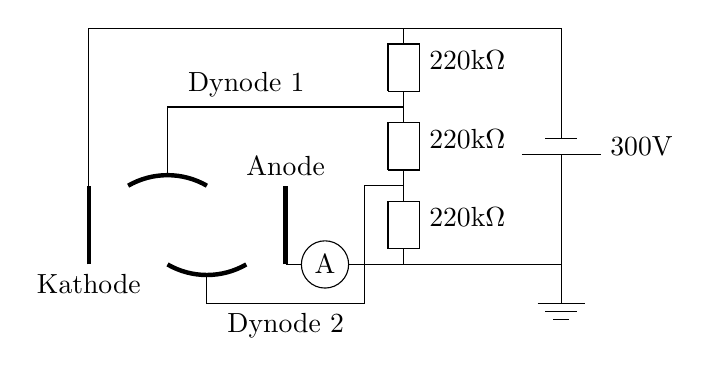
\begin{tikzpicture} 
\draw [ultra thick] (0,0)--(0,1);
\node [below] at (0,0) {Kathode}; 
\draw (0,1)--(0,3)--(6,3)--(6,1.6);
\draw [ultra thick] (1.5,1) arc [radius=1, start angle=60, end angle= 120];
\draw (1,1.15)--(1,2)--(4,2);
\node [above] at (2,2) {Dynode 1}; 
\draw [ultra thick] (1,0) arc [radius=1, start angle=240, end angle= 300];
\draw (1.5,-.15)--(1.5,-.5)--(3.5,-.5)--(3.5,1)--(4,1);
\node [below] at (2.5,-.5) {Dynode 2}; 
\draw [ultra thick] (2.5,0)--(2.5,1);
\node [above] at (2.5,1) {Anode};
\draw (3,0) circle [radius=0.3];
\node [] at (3,0) {A};
\draw (2.5,0)--(2.7,0);
\draw (3.3,0)--(6.0,0)--(6.0,1.4);
\draw (3.8,.2)--(4.2,.2)--(4.2,.8)--(3.8,.8)--(3.8,.2);
\node [right] at (4.2,.6) {220k$\Omega $};
\node [right] at (4.2,1.6) {220k$\Omega $};
\node [right] at (4.2,2.6) {220k$\Omega $};
\node [right] at (6.5,1.5) {300V};
\draw (3.8,1.2)--(4.2,1.2)--(4.2,1.8)--(3.8,1.8)--(3.8,1.2);
\draw (3.8,2.2)--(4.2,2.2)--(4.2,2.8)--(3.8,2.8)--(3.8,2.2);
\draw (4,0)--(4,.2);
\draw (4,.8)--(4,1.2);
\draw (4,1.8)--(4,2.2);
\draw (4,2.8)--(4,3);
\draw (5.5,1.4)--(6.5,1.4);
\draw (5.8,1.6)--(6.2,1.6);
\draw (6,0)--(6,-.5);
\draw (5.7,-.5)--(6.3,-.5);
\draw (5.8,-.6)--(6.2,-.6);
\draw (5.9,-.7)--(6.1,-.7);
\end{tikzpicture}
\caption{\label{PMT-schema}Een PMT-buis met twee dynodes} 
\end{figure}

Als er geen licht op de kathode valt, worden hier geen elektronen
vrijgemaakt en loopt er geen stroom naar of van de kathode. 


\paragraph{1 }

\textit{Leg uit of de stroom naar de kathode zou gaan of dat deze
van de kathode zou komen als er licht op de kathode valt.}

Er worden geen elektronen bij beide dynodes vrijgemaakt, hier loopt
dus ook geen stroom. De enige stroomkring is de stroomkring door de
in serie geschakelde weerstanden. Voor deze stroomkring kunnen we 
volgens Kirchhoff zeggen dat: 

\begin{equation}
\begin{array}{c} 
n\\ 
\sum\\ 
i=1
\end{array}
U_{i}=0
\end{equation}


\paragraph{2}

\textit{Stel de vergelijking voor de spanning in deze stroomkring
op volgens Kirchhoff en bereken de stroom door deze kring.}


\paragraph{3}

\textit{Bereken de spanningen tussen de aarde en de kathode, de eerste
dynode, de tweede dynode en de anode.}

De kathode wordt hierna verlicht. De kathodestroom wordt 6,33nA.
Als een elektron van de kathode op de eerste dynode valt, worden er
twee extra elektronen vrijgemaakt. Dit gebeurt ook met de elektronen
bij de tweede dynode.


\paragraph{4}

\textit{Bereken de stromen door de eerste en tweede dynode en de stroom
door de anode.}

Deze stromen worden afgetakt van de stroomkring door de weerstanden. 
Voor iedere punt waar stroom wordt afgetakt geldt:

\begin{equation}
\begin{array}{c} 
n\\ 
\sum\\ 
i=1
\end{array}
I_{i}=0
\end{equation}

\paragraph{5}

\textit{Bereken de stromen door de weerstanden. De stroom door de weerstand 
kan als $I_{bat}$ worden geschreven. Dit is de enige variabele.}

\paragraph{6}

\textit{Bereken met de spanningen over de weerstanden de spanning op de kathode, de dynodes en de anode
als de PMT-buis wordt verlicht. ($I_{kathode}=6,33$nA)}

In de praktijk zitten er in PMT-buizen meer dynodes. De PMT-buizen
voor de detectoren voor kosmische straling op het dak van de school
hebben 10 dynodes.


\paragraph{7}

\textit{Bereken hoeveel de stroom nu in het totaal versterkt wordt.}


\section{De werking van een dynode}

De werking van een dynode is met energie uit te leggen. Op de eerste
dynode vallen elektronen die afkomstig zijn van de kathode. Zoals
bekend is de energie van een elektron te bepalen met de spanning en
de lading.

\begin{equation}
U=\frac{E}{q}
\end{equation}


We gaan uit van een spanning tussen de kathode en de eerste dynode van 100V.


\paragraph{8}

\textit{Bereken de verandering van de energie van het elektron als dit van de kathode
naar de eerste dynode gaat.}

Tussen de kathode en de eerste dynode wordt elektrische energie omgezet
in bewegingsenergie $\left(E=\frac{1}{2}mv^{2}\right)$.


\paragraph{9}

\textit{Bereken de snelheid van het elektron bij de eerste dynode
als we de snelheid bij de kathode mogen verwaarlozen.}

De energie van het elektron bij de eerste dynode wordt gebruikt om
elektronen uit het metaal te botsen.


\paragraph{10}

\textit{Beredeneer wat er met de versterking gebeurd als we de spanning
tussen kathode en anode verhogen.}
\end{document}
